%%%%%%%%%%%%%%%%%%%%%%%%%%%%%%%%%%%%%%%%%%%%%%%%%%%%%%%%%%%%%%%
%
% Welcome to Overleaf --- just edit your LaTeX on the left,
% and we'll compile it for you on the right. If you open the
% 'Share' menu, you can invite other users to edit at the same
% time. See www.overleaf.com/learn for more info. Enjoy!
%
%%%%%%%%%%%%%%%%%%%%%%%%%%%%%%%%%%%%%%%%%%%%%%%%%%%%%%%%%%%%%%%
% Author: Izaak Neutelings (September 2020)
\documentclass[border=3pt,tikz]{standalone}
\usepackage{amsmath}
\usepackage{tikz}
\usepackage{physics}
\usetikzlibrary{calc}
\tikzset{>=latex} % for LaTeX arrow head
\usepackage{xcolor}
\colorlet{veccol}{green!45!black}
\colorlet{myred}{red!90!black}
\colorlet{myblue}{blue!90!black}
\colorlet{mypurple}{blue!50!red!80!black!80}
\tikzstyle{vector}=[->,very thick,veccol]
\usetikzlibrary{arrows.meta}
\tikzstyle{thin arrow}=[dashed,thin,-{Latex[length=4,width=3]}]

\begin{document}


% TWO VECTORS SUM
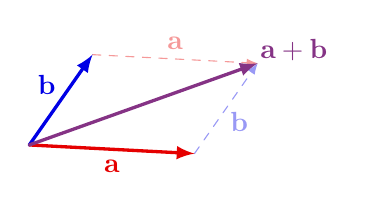
\begin{tikzpicture}[line cap=round]
  \coordinate (O) at (0,0);
  \coordinate (A) at ( -3:2.1);
  \coordinate (B) at ( 55:1.4);
  \coordinate (A+B) at ($(A)+(B)$);
  
  \draw[vector,thin arrow,myred!40] (B) -- (A+B) node[midway,above] {$\vb{a}$};
  \draw[vector,thin arrow,myblue!40] (A) -- (A+B) node[midway,below right=-2] {$\vb{b}$};
  
  \draw[vector,myred] (O) -- (A) node[midway,below] {$\vb{a}$};
  \draw[vector,myblue] (O) -- (B) node[midway,above left=-2] {$\vb{b}$};
  \draw[vector,mypurple] (O) -- (A+B) node[above right=-3] {$\vb{a}+\vb{b}$};
\end{tikzpicture}


% VECTORS
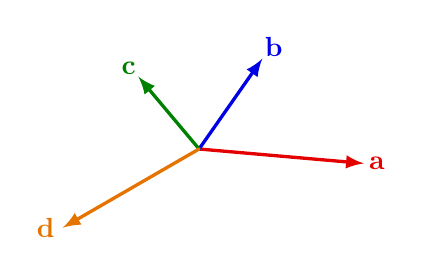
\begin{tikzpicture}[line cap=round]
  \coordinate (O) at (0,0);
  \coordinate (A) at ( -5:2.1);
  \coordinate (B) at ( 55:1.4);
  \coordinate (C) at (130:1.2);
  \coordinate (D) at (210:2.0);
  \draw[vector,myred] (O) -- (A) node[right=-2] {$\vb{a}$};
  \draw[vector,myblue] (O) -- (B) node[above right=-3] {$\vb{b}$};
  \draw[vector,green!50!black] (O) -- (C) node[above left=-3] {$\vb{c}$};
  \draw[vector,orange!90!black] (O) -- (D) node[left=-1] {$\vb{d}$};
\end{tikzpicture}


% VECTOR SUM
\begin{tikzpicture}[line cap=round]
  \draw[vector,myred] (O) -- (A) node[below left=0] {$\vb{a}$};
  \draw[vector,myblue] (A) --++ (B) node[below right=-3] {$\vb{b}$};
  \draw[vector,green!50!black] (A)++(B) --++ (C) node[above=1,right=2] {$\vb{c}$};
  \draw[vector,orange!90!black] (A)++(B)++(C) --++ (D) node[above=2] {$\vb{d}$};
  \draw[vector,<-,blue!50!black] (A)++(B)++(C)++(D) -- (O)
    node[midway,left=1,scale=0.9] {$\vb{a}+\vb{b}+\vb{c}+\vb{d}$};
\end{tikzpicture}


\end{document}
